\chapter{Estado del arte}


\section{¿Qué es una ECU?}


Una ECU \textit{Electronic Control Unit} es un sistema empotrado, que consta de un microcontrolador especializado en la automoción. [1] (embitel.com) Permite, junto con el software y los protocolos de comunicación, y el conjunto de sensores y actuadores, controlar los sistemas eléctricos y subsistemas en un vehículo para su correcto funcionamiento. 
Esencialmente se encarga de recibir la información que le aportan los sensores acerca del entorno, procesar esa información para completar diversas tareas y, en muchos casos, enviar las directrices que se requieren a los actuadores de los componentes.\newline


\begin{figure}[h]
    \centering
    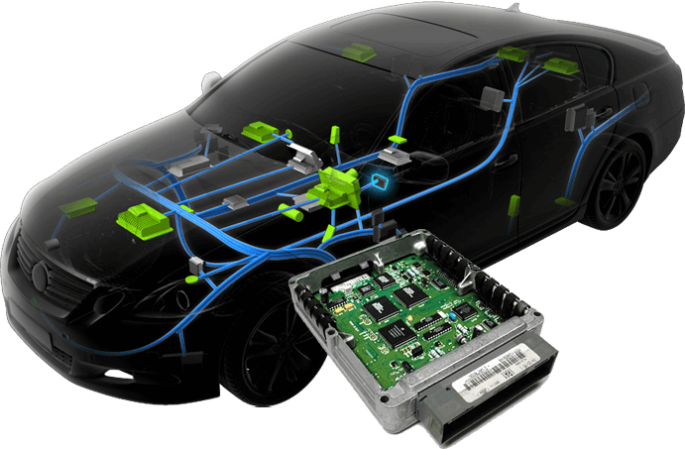
\includegraphics[width=0.5\textwidth]{imagenes/ECU_autotechdrive.png}
    \caption{Imagen de una ECU y su impacto en un vehículo. Extraído de: []}
\end{figure}


\subsection{Evolución e historia de la gestión de datos los vehículos}

Las siglas ECU no siempre han tenido el mismo significado. Inicialmente, cuando se comenzaron a utilizar (en torno a los años setenta), era para hablar de la unidad de control del motor \textit{\textbf{Engine Control Unit}}. Podemos desgajar los grandes cambios en lo siguiente[4]:

\begin{itemize}

    \item \textbf{Años 70} - Inicialmente eran dispositivos extremadamente simples, que solamente controlaban un par de solenoides en el \textbf{carburador}, el encargado de preparar la mezcla de aire y combustible en motores de gasolina, de manera que el vehículo pudiera obtener la máxima potencia de salida de la manera más eficiente.

    \begin{figure}[h]
        \centering
        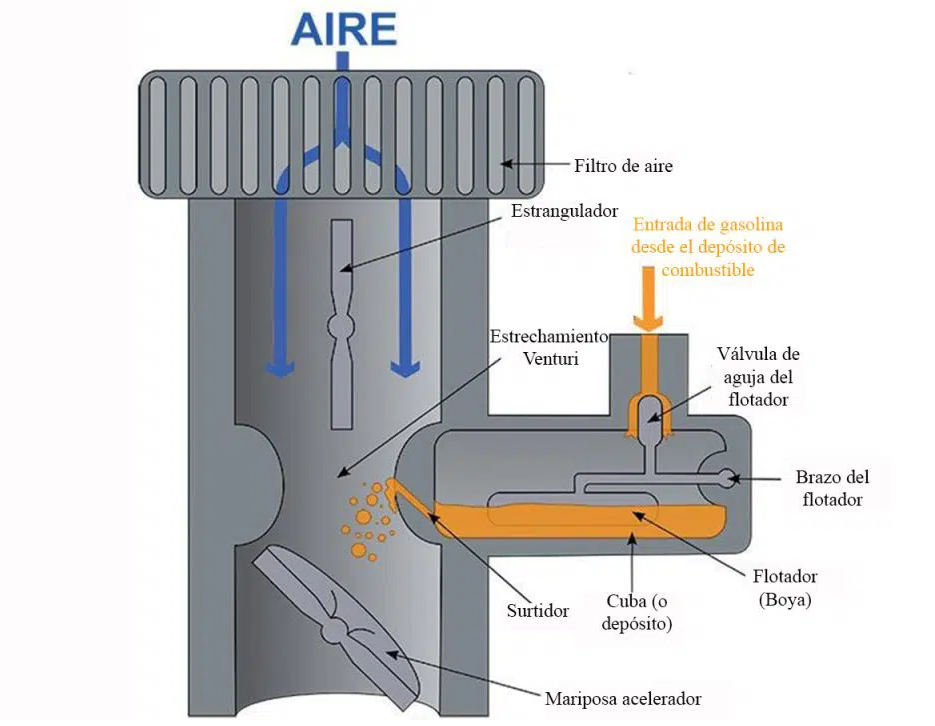
\includegraphics[width=0.5\textwidth]{imagenes/esquema_carburador.png}
        \caption{Imagen simplificada de un carburador sus partes. Extraído de: [5]}
    \end{figure}
 
    \item \textbf{Años 80} - En esta época se comenzaron a utilizar los \textbf{reguladores de presión de combustible}, un componente que busca controlar y mantener constante la presión del combustible. Permitió a los fabricantes de vehículos tener mayor control a la hora de no dañar otros componentes, tales como inyectores o los conductos del sistema en general [5]. En este punto, la unidad de control del motor ya era la principal responsable de los sistemas de combustión. También comenzaron a utilizar el \textbf{Control de Lambda} para modificar parámetros de la misma, y alcanzar una mayor eficiencia.

    \begin{figure}[h]
        \centering
        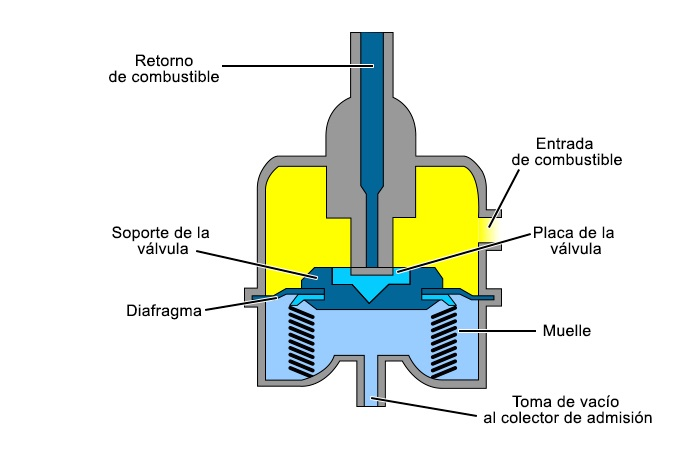
\includegraphics[width=0.6\textwidth]{imagenes/esquema_rpc.png}
        \caption{Imagen simplificada de un regulador de combustible y sus partes. Extraído de: [7]}
    \end{figure}


    \item \textbf{Años 90} - Las ECUs añadieron un conjunto de medidas para mejorar la seguridad en el vehículo, siendo el \textbf{ABS ó Antiblockiersystem} la más relevante. Esta tecnología, aún en uso en los vehículos actuales, se encarga de variar la fuerza de frenado al detectar mediante sensores de revoluciones en las ruedas, evitando así que estas se bloqueen y perdamos el control del vehículo. El uso de las ECUs se extiende hacia los motores diésel, teniendo un papel esencial en el desarrollo de los vehículos turbodiésel.

    \begin{figure}[h]
        \centering
        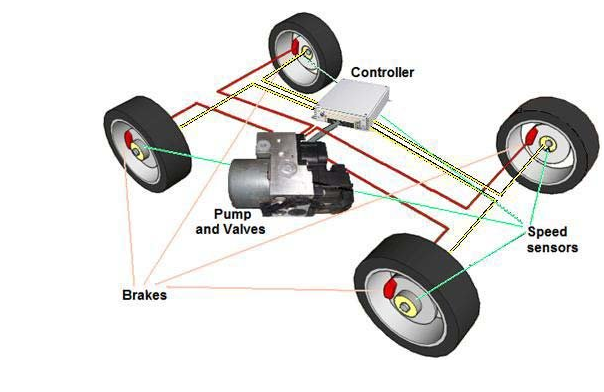
\includegraphics[width=0.5\textwidth]{imagenes/esquema_abs.png}
        \caption{Imagen simplificada del ABS y sus partes. Extraído de: [8]}
    \end{figure}
    
 
    \item \textbf{Años 2000} - Las unidades de control comienzan a incluir la tecnología \textit{\textbf{drive-by-wire}}, un formalismo para definir la sustitución de controles mecánicos tradicionales por sistemas electrónicos [9], así como también se añade control del turbo y sistemas para minimizar emisiones y cumplir con los protocolos pertinentes.
       

    \begin{figure}[h]
        \centering
        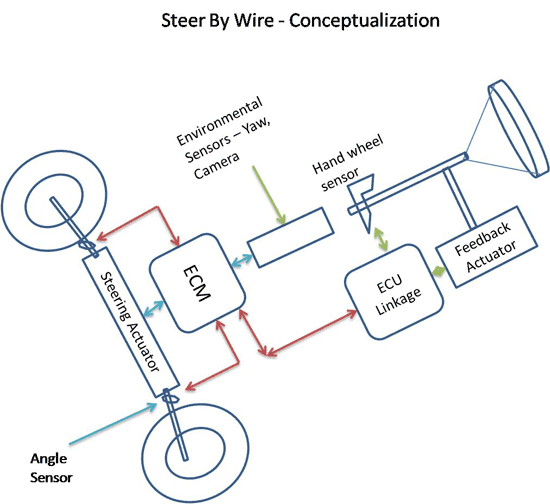
\includegraphics[width=0.5\textwidth]{imagenes/esquema_dbw.png}
        \caption{Conceptualización del sistema \textit{drive-by-wire}. Extraído de: [10]}
    \end{figure}
          

    \item \textbf{Años 2010-Actualidad} - La centralita del motor controla todo el sistema de mezcla del combustible, emisiones, refrigeración y sistemas de aceleración del vehículo. Dejan de ser dispositivos simples, ahora tienen cientos de entradas, decenas de sensores, y forman parte de un conjunto de ECUs (ya utilizando la acepción actual del término: \textit{Electronic Control Unit}), cada una focalizada en un conjunto de tareas, yendo desde el propio control del motor, hasta los sistemas de infoentretenimiento del vehículo. 
       

    \begin{figure}[h]
        \centering
        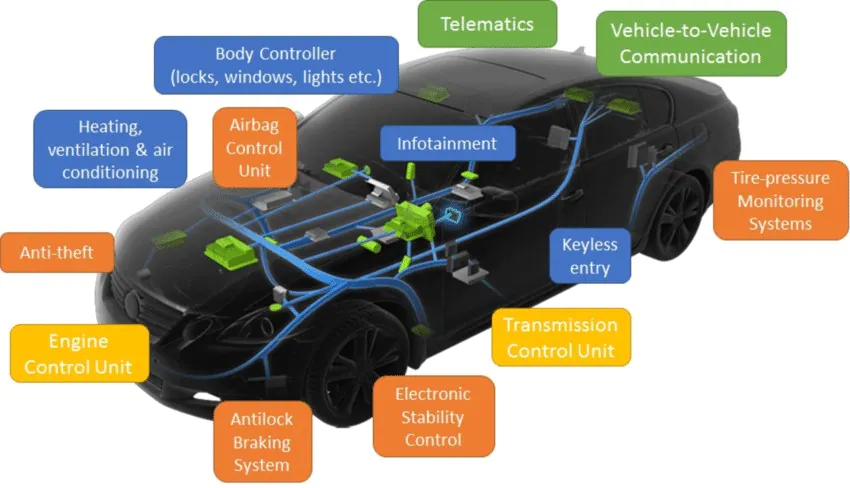
\includegraphics[width=0.5\textwidth]{imagenes/ECU_autotechdrive_completa.png}
        \caption{Representación de las distintas ECUs que controlan un vehículo. Extraído de: [11]}
    \end{figure}
\end{itemize}

\newpage
       
\begin{figure}[h]
    \centering
    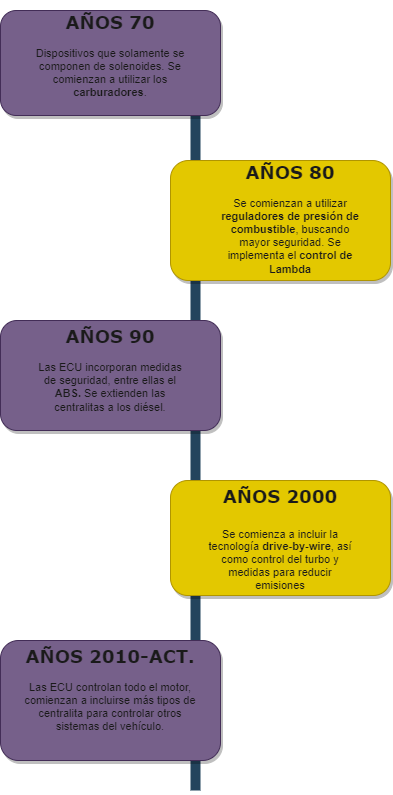
\includegraphics[width=0.54\textwidth]{imagenes/timeline_ECU.png}
    \caption{Linea temporal de las ECUs. Elaboración propia}
\end{figure}


\newpage


\subsection{Tipos de ECUs}
Como se ha visto en el anterior apartado, el significado de las siglas ECU ha variado con el tiempo, refiriéndose ahora a cada uno de los sistemas que controlan diversas partes del vehículo. A grandes rasgos, podemos hablar de los siguientes tipos[12]
\begin{itemize}
    \item \textbf{BCM - \textit{Body Control Module}}: Esta unidad controla tareas de índole variada, desde las luces, hasta el mecanismo de las ventanas, los retrovisores (si son motorizados), limpiaparabrisas, etc.
    \item \textbf{CCM - \textit{Climate Control Module}}: Este módulo se encarga de gestionar toda la climatización, temperatura, potencia de la bomba del aire acondicionado y calefacción.
    \item \textbf{ECM - \textit{Engine Control Module}}: Conocido antiguamente como ECU. Se encarga de gestionar todas las tareas del motor, ya mencionadas en el apartado anterior.
    \item \textbf{EBCM - \textit{Electronic Brake Control Module}}: Si el vehículo tiene un freno electrónico, este módulo es el encargado de su correcto funcionamiento.
    \item \textbf{ICM - \textit{Infotainment Control Module}}: Esta ECU controla todo lo relacionado con el infoentretenimiento, mayormente centrado en la tableta integrada del vehículo.
    \item \textbf{PSM - \textit{Power Steering Module}}: Este módulo gestiona las tareas que requiere la dirección para funcionar. Tiene una gran importancia, debido al uso de la dirección asistida en los vehículos actuales.
    \item \textbf{PCM - \textit{Powertrain Control Module}}: Esta ECU se encarga de la interconexión e interacción de los componentes que forman el \textbf{tren motriz}, el sistema que permite que la energía generada se transforme en movimiento sobre el terreno. Gestiona lo relacionado con el motor, la transmisión, los ejes, los diferenciales y la dirección del vehículo. 
    \item \textbf{SCM - \textit{Suspension Control Module}}: El objetivo de este módulo es controlar los sistemas de suspensión del vehículo.
    \item \textbf{TCM - \textit{Transmission Control Module}}: Este módulo controla todo lo relacionado con la transmisión, las marchas, el cambio y la entrega de potencia en las ruedas.
\end{itemize}
\newpage
\section{Diseño hardware de las centralitas}

Para tener un funcionamiento acorde a su importancia, las ECUs están constituidas por varios componentes, que serán los que se estudiarán en este apartado.

\begin{figure}[h]
    \centering
    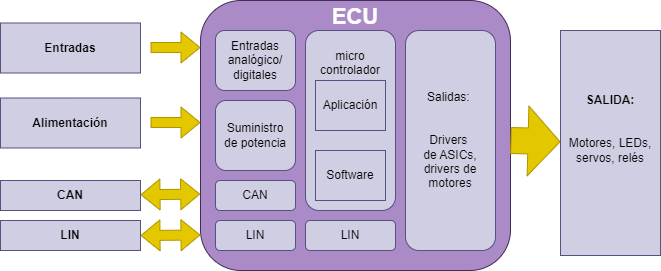
\includegraphics[width=0.70\textwidth]{imagenes/ECU_hardware.png}
    \caption{Componentes hardware de una ECU. Elaboración propia}
\end{figure}

\subsection{Procesador central}
El microcontrolador es la piedra angular de una centralita. Su tarea varía según el tipo de ECU que lo contenga, pero generalmente consiste en realizar todo el procesamiento de datos, así como hacer uso de las lineas de comunicación para recibir y enviar información a los subsistemas requeridos. \newline
Estos microcontroladores pueden interaccionar entre sí, aun perteneciendo a diferentes centralitas, por medio de \textbf{multiplexación}, así como también de los buses o protocolos de comunicación. Esta relación permite a un sistema valerse de otros para realizar una tarea, véase el siguiente ejemplo: 

\begin{enumerate}
    \item El usuario nota que hace demasiado calor en el vehículo, por lo que decide cambiar la temperatura en la tableta central del vehículo.
    \item Este sistema, controlado por el \textbf{ICM} (\textit{Infotainment Control Module}), recibe la entrada del usuario y envía una señal a la ECU que se encarga de la climatización (\textbf{CCM}).
    \item El módulo de climatización recibe la entrada y envía una señal a sus actuadores para encender el aire acondicionado.
\end{enumerate}


Respecto a la arquitectura del microcontrolador, existen diversas opciones, todas (o casi todas) ellas oscilando entre los 8 bits y los 32 bits, siendo estos últimos los más extendidos con el \textbf{Infineon Tri-core Microcontroller[19]}. Este micro se encarga de gestionar todas las tareas de emisiones y sistemas de combustión. 

La elección entre un chip u otro también se hace en base a las necesidades del sistema, puesto que algunos, como el tren de potencia y el control del vehículo requieren de un menor tiempo de respuesta y un mayor rendimiento, mientras que el infoentretenimiento no tiene tanta restricción al ser un \textbf{sistema de tiempo real blando} (incumplir el límite acotado del tiempo de respuesta no ocasiona daños personales o materiales)

\subsection{Memoria}

En una ECU, normalmente existen tres tipos de memoria, \textbf{ROM}, \textbf{RAM} y \textbf{PROM/EEPROM}. Cada una tiene un objetivo específico y unas restricciones asociadas:

\begin{itemize}
    \item \textbf{Memoria no volátil}: La ECU almacena en este tipo de memoria información que no se debe borrar una vez se apague el vehículo, como los datos del sistema y los del usuario (configuraciones, perfiles de conducción, etcétera.).
    \begin{itemize}
        \item \textbf{ROM}: Almacena información de programación que solo puede leer la ECU. Es de solo lectura, y su existencia es de vital importancia para el funcionamiento del vehículo.
        \item \textbf{PROM/EEPROM}: Este tipo de memoria está hecha por el fabricante, con el objetivo de ajustarse a la aplicación de la transmisión, motor y demás piezas fundamentales del vehículo. Mientras que la PROM no se puede reprogramar, la EEPROM (\textit{Electrically Erasable Programmable Read-Only Memory}) permite al usuario o al operario reprogramarla con un dispositivo especial. 
    \end{itemize}
    \item \textbf{Memoria volátil}: La ECU utiliza esta memoria para almacenar datos temporales, no mantiene la información entre reinicios.
    \begin{itemize}
        \item \textbf{RAM}: Esta memoria permite almacenar datos temporales de las entradas, códigos de error para el diagnóstico, y resultados de cómputos para trabajar con los actuadores. Tiene un tiempo de acceso mucho menor a las \textbf{NVM} (\textit{Non-Volatile Memory}).
    \end{itemize}
\end{itemize}

\subsection{Sensores}

Los sensores tienen un papel esencial en el diseño hardware de las ECU, dando información de los sistemas del vehículo al microcontrolador para su monitorización. 


\section{La ECU en los vehículos: El mejor amigo del conductor}

El ser humano ha hecho grandes avances en la tecnología, y esto no podría ser menos en los vehículos. Las ECU que, como se ha visto en el apartado anteror, inicialmente no tenían tanta importancia, ahora se han convertido en algo fundamental para nosotros. Estas centralitas, que antiguamente servían únicamente para gestionar la inyección de combustible en el el motor, ahora tienen multitud de utilidades para cada una de las partes del vehículo.

Gracias a estos sistemas, podemos obtener desde una mayor eficiencia en el uso de la fuente de energía (ya sea combustible fósil o electricidad), un control más específico de los mapas motor para mayor potencia, recolección de datos relevantes del vehículo, e incluso algunas mejoras \textit{Quality of Life (QoL)} que nos permitan una conducción más cómoda. 

Muchos de estos sistemas no solamente inciden en la eficiencia y comodidad, sino también en la seguridad del conductor y de los pasajeros abordo. Algunas de las medidas más relevantes, que vamos a categorizar entre activas y pasivas, son las siguientes[11]:

\begin{enumerate}
    \item \textbf{Seguridad activa} - Conjunto de medidas que proporcionan mayor estabilidad al vehículo, buscando evitar el accidente a priori.
    \begin{itemize}
        \item \textit{Luces adaptativas}: Esta tecnología se basa en el uso de una matriz de LEDs en las luces delanteras, al contrario de la tradicional bombilla incandescente usada anteriormente. Los beneficios de este diseño son múltiples, pues permite modificar el haz de luz para evitar posibles deslumbramientos a otros usuarios de la vía, así como también adaptarse a las condiciones de la carretera, e iluminar más eficazmente el trazado.


     
        \item \textit{Control de crucero adaptativo (ACC)}: Permite mantener una velocidad designada por el conductor, variando cuando sea necesario por las condiciones del tráfico. Esta tecnología supone una gran ayuda en el caso de que exista una distracción del conductor. Puede funcionar junto a un sistema de detección de señales para no sobrepasar la velocidad máxima permitida en esa vía.
    
        \item \textit{Sistema de alerta de tráfico y evasión de colisión (TCAS)}: Este sistema tiene como tarea principal la detección de eventos en el tráfico que puedan causar un accidente, reaccionando (normalmente accionando de manera automática el freno), o advirtiendo al conductor para que sea él el que realice la acción pertinente para evitarlo.

        \item \textit{Sistema de detección de cansancio}: Algunos fabricantes [14] comienzan a implementar esta tecnología que, mediante sensores en la posición del conductor, o analizando su conducción, permite detectar si existen síntomas de cansancio o distracción. Normalmente muestran un aviso que se repite de manera continuada hasta que se realiza una parada. 
\end{itemize}

\begin{figure}[h]
    \centering
    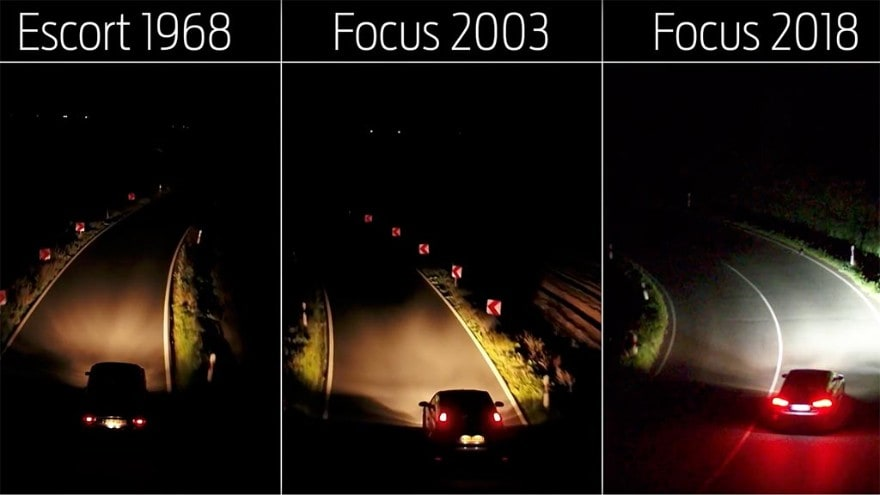
\includegraphics[width=0.7\textwidth]{imagenes/adaptive_lights.png}
    \caption{Comparación de la iluminación en los vehículos tras los años. Extraído de: [14]}
\end{figure}


    \item \textbf{Seguridad pasiva} - Conjunto de medidas que actúan una vez ha sucedido el accidente o el mal funcionamiento. Tienen el objetivo de minimizar los daños.

    \begin{itemize}
        \item \textit{Sistema de sensor de ocupación}: Permite detectar qué asientos están siendo utilizados, y comprobar el peso para saber si el ocupante es un niño o un adulto. Normalmente se utiliza para accionar el airbag si fuera necesario, y la altura a la que hacerlo.

        \item \textit{Notificación de colisión automática}: Este sistema envía un aviso a los servicios de emergencia de su localicación para que sea posible una intervención rápida.[16]
    \end{itemize}
\end{enumerate}




\section{La necesidad de un RTOS en las ECUs}

2.2.2 Real-Time Operating System
The general structure of a more recent (but not fully modern) ECU follows a model
similar to the main loops outlined in 2.2.1, but these loops are often distributed across
multiple cores with a more complex scheduling system. This requires the use of a realtime-operating-system (RTOS) to schedule, manage, and distribute the cores of the CPU so
that each function can execute on-time. This allows for important sensor reading functions,
health checking functions, and fuel injection functions to be ran concurrently, increasing
their speed and response time and greatly increasing their safety and optimizing their performance. Several contemporary open-source ECUs are implemented on top of an RTOS
to schedule necessary tasks, with a notable one being rusEfi which was built on top of the
open-source platform FreeRTOS[5]

\section{Futuras tendencias en el campo de las ECU: ¿Qué podemos esperar?}

\section{Código Abierto, Software Libre y Licencias}

El software libre y sus licencias \cite{gplv3} ha permitido llevar a cabo una expansión del
aprendizaje de la informática sin precedentes.

\section{Conclusiones}